\documentclass[12pt]{article}
\usepackage{amsmath, amssymb, amsthm}
\usepackage{mathtools}
\usepackage{graphicx}
\usepackage{float}
\usepackage{hyperref}
\usepackage{xcolor}
\usepackage{listings}
\usepackage{geometry}
\usepackage{algorithm}
\usepackage{algpseudocode}
\usepackage{tikz}
\usepackage{longtable}
\usepackage{circuitikz}
\usepackage{comment}
\usepackage[section]{placeins}

% Page Setup
\geometry{a4paper, margin=1in}

% Custom Commands
\newcommand{\vecb}[1]{\mathbf{#1}}
\newcommand{\brak}[1]{\ensuremath{\left(#1\right)}}
\newcommand{\cbrak}[1]{\ensuremath{\left\{#1\right\}}}
\newcommand{\abs}[1]{\left\vert#1\right\vert}
\newcommand{\norm}[1]{\left\lVert#1\right\rVert}

\begin{document}
\title{Analyzing Response of RC Circuits against Square Wave Voltage Source with Varying Time Period}
\author{Abhimanyu Koushik \brak{\text{EE24BTECH11024}},\\Agamjot Singh \brak{\text{EE24BTECH11002}}\\IIT Hyderabad}
{\let\newpage\relax\maketitle}
\setlength{\intextsep}{10pt} % Space between text and floats
\bibliographystyle{IEEEtran}

\section*{Abstract}
This report examines the response of an RC circuit to a square wave input of time period $T$, with particular focus on three cases: $T \gg RC$, $T = RC$, and $T \ll RC$. The behavior of the output voltage across the capacitor is analyzed in each case, highlighting the effect of the relationship between the time constant $RC$ and the period of the input signal.

\section{Introduction}
RC circuits, consisting of a resistor and a capacitor in series, exhibit dynamic behavior when subjected to time-varying inputs. The response of such circuits is governed by their time constant $\tau = RC$. When driven by a square wave input, the circuit's output depends on the interplay between the time constant and the time period $T$ of the square wave. This document explores the circuit's response for three distinct scenarios.

\section{Theory}
\begin{figure}[h!]
    \centering
    \begin{circuitikz}
        % Define circuit components
        \draw 
        (0,0) node[ground]{} % Ground symbol
        (0,0) to[square voltage source, l=\(5V\)] (0,3) % Square wave voltage source
        to[R, l=$R$] (3,3) % Resistor
        to[C, l=$C$] (3,0) % Capacitor
        -- (0,0); % Closing the circuit
    \end{circuitikz}
    \caption{RC Circuit with a 5V Square Wave Input}
\end{figure}
The reactance of a capacitor with capacitance $C$ is given by 
\begin{align}
	\chi_{C} = \frac{1}{j\omega C}
\end{align}
Where $j = \sqrt{-1}$ and $\omega$ is the Angular frequency of input voltage\newline
The voltage across capacitor in an RC series circuit with sine input is given by
\begin{align}
	V_{\text{in}} &= V_R + V_C\\
	V_R &= iR\\
	V_C &= i\chi_{C}\\
	V_{\text{in}} &= iR + i\chi_C\\
	i &= \frac{V_{\text{in}}}{R+\chi_C}\\
	V_C &= \frac{V_{\text{in}}}{R+\chi_C}\chi_C\\
	V_C &= \frac{V_{\text{in}}}{1+j\omega RC}
\end{align}
The transfer function is given $H\brak{j\omega} = \frac{V_{\text{out}}}{V_\text{in}}$. For the given circuit
\begin{align}
	H\brak{j\omega} &= \frac{1}{1+j\omega RC}
\end{align}
The bode plot for amplitude is given by plotting $y = 20\log(\abs{H(j\omega)})$ against $x = \log(\omega)$.
\begin{align}
	y &= 20\log(\abs{H(j\omega)})\\
	y &= 20\log(\frac{1}{\sqrt{1+(\omega RC)^2}})\\
	y &= -10\log(1+(\omega RC)^2)\\
	y &= -10\log(1+10^{2x}R^2C^2)
\end{align}
The function to be plotted in bode plot for the Amplitude will be 
\begin{align}
	y = -10\log(1+10^{2x}R^2C^2)
\end{align}
\section{Procedure}

\begin{enumerate}
    \item Connect the function generator to the oscilloscope using BNC cables to the probes of the oscilloscope's probes.
    The ground (black) wire of the BNC cable is the ground which is to be connected to the ground of the probe (which is sticking out). The live (red) wire of the BNC cable is to be connected to the probe.
    \item Input a square wave which oscillates between the values 5$V$ and 0$V$ using the function generator. Set the time period to $T$.
    \item Set the display mode to $X - T$ and align the phase after each change in the \textbf{Inter CH} dropdown.
    \item Measure the Voltage drop across the capacitor using the probe. Capture the wave which is being displayed on the screen. It is the graph of the response in steady state.
    \item To measure the transient part for the first 5 cycles, set the function generator to burst mode, generate a burst of 5 cycles. Record the event using the \textbf{Single} event option.
    \item Repeat the same for different values of $T$.
\end{enumerate}

\section{Numerical Solution Using the Trapezoidal Method}
To solve the governing differential equation numerically, we employ the trapezoidal method. The Python implementation simulates the circuit response to a square wave input.\newline
According to trapezoidal rule
\begin{align}
  y_{n+1}&=y_n+\frac{1}{2}h\brak{f(t_n,y_{n}) + f(t_{n+1},y_{n+1})}\\
  f(t_n, y_n) &= \frac{1}{RC}(V_{in}(t_n) - V_{C}(y_n))\\
  V_{C}(y_{n+1})&=V_{C}(y_n)+\frac{1}{2}h (\frac{1}{RC}(V_{in}(t_n) - V_{C}(y_n))+\frac{1}{RC}(V_{in}(t_{n+1}) - V_{C}(y_{n+1})))\\
  V_{C}(y_{n+1})&=V_{C}(y_n)+\frac{h}{2RC}((V_{in}(t_n) - V_{C}(y_n))+(V_{in}(t_{n+1}) - V_{C}(y_{n+1})))\\
  (1+\frac{h}{2RC})(V_{C}(y_{n+1})) &= V_C(y_n)+\frac{h}{2RC}(V_{in}(t_n)+V_{in}(t_{n+1})- V_{C}(y_n))
\end{align}
We will get the expression
\begin{align}
	(V_{C}(y_{n+1})) &= \frac{V_C(y_n)+\frac{h}{2RC}(V_{in}(t_n)+V_{in}(t_{n+1})- V_{C}(y_n))}{1+\frac{h}{2RC}}
\end{align}
\subsection{Explanation of the Code}
The Python code above simulates the response of an RC circuit to a square wave input. Key steps include:
\begin{itemize}
    \item Defining circuit parameters such as resistance, capacitance, and time step size.
    \item Generating a square wave function for the input voltage.
    \item Implementing the trapezoidal method to numerically integrate the differential equation governing the RC circuit.
    \item Updating the capacitor voltage iteratively using past and present input values.
    \item Plotting the results to visualize the circuit response.
\end{itemize}
\section{Analysis}
\subsection{Case 1: $T \gg RC$}
When the period of the square wave is much greater than the time constant ($T \gg RC$), the capacitor has sufficient time to fully charge and discharge during each half-cycle. The output voltage $V_C(t)$ closely follows the input signal, with exponential transitions between $V_0$ and $-V_0$. The response can be expressed as:
\begin{align}
    V_C(t) = V_0 \left(1 - e^{-t/(RC)}\right) \quad \text{(during charging)},
\end{align}
\begin{align}
    V_C(t) = -V_0 \left(1 - e^{-t/(RC)}\right) \quad \text{(during discharging)}.
\end{align}
\newpage
Continous $\hspace{\fill}$ Simulation $\hspace{1in}$
\begin{figure*}[!htb]
    {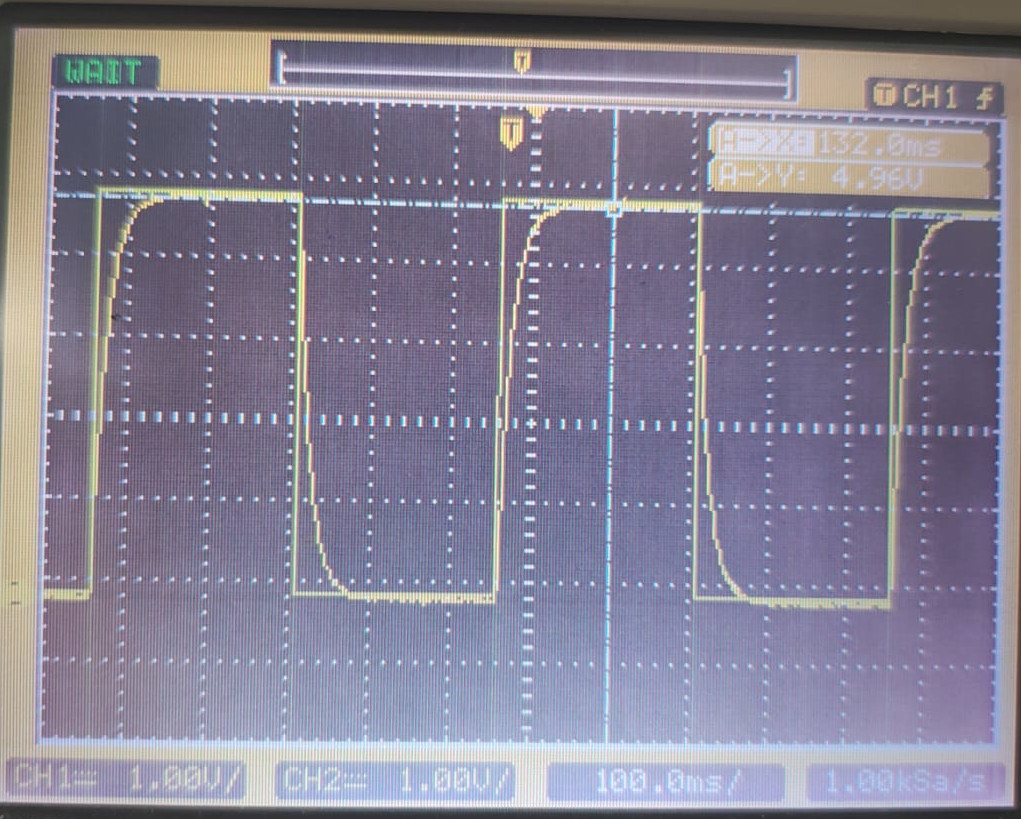
\includegraphics[ width=0.5\textwidth]{./figs/greater_cont_crop.jpeg}}
    \hspace{\fill}
    {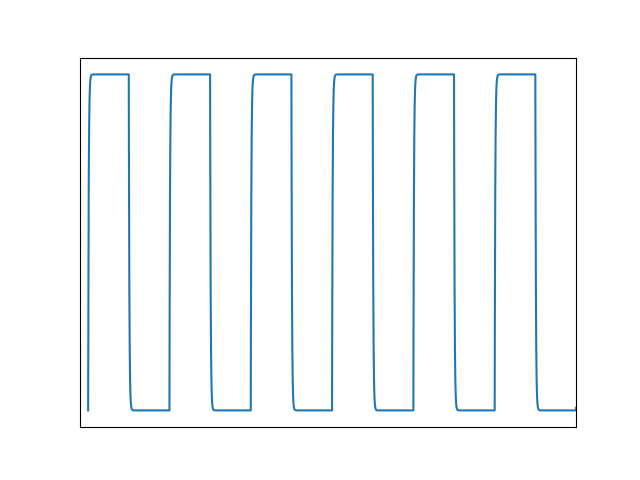
\includegraphics[ width=0.5\textwidth]{./figs/greater_cont_sim.png}}
    \caption{$T = 0.5 s\gg RC$}
\end{figure*}

Burst \brak{\text{5 cycles}} $\hspace{\fill}$ Simulation $\hspace{1in}$
\begin{figure*}[!htb]
    {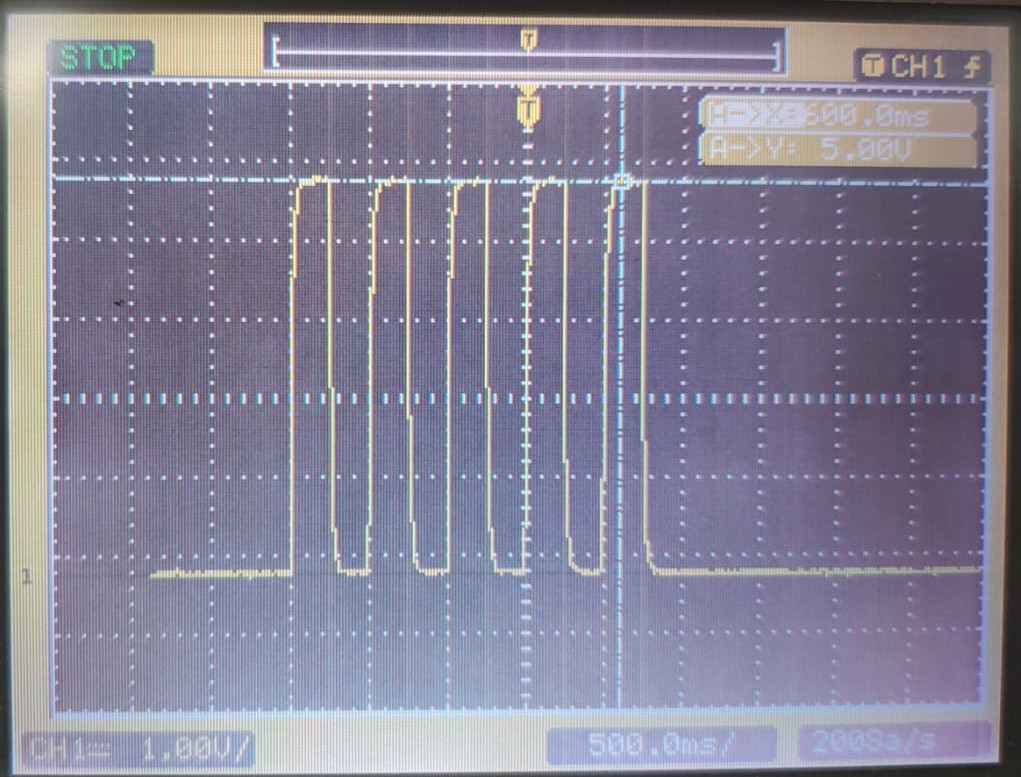
\includegraphics[ width=0.5\textwidth]{./figs/greater_burst_crop.jpeg}}
    \hspace{\fill}
    {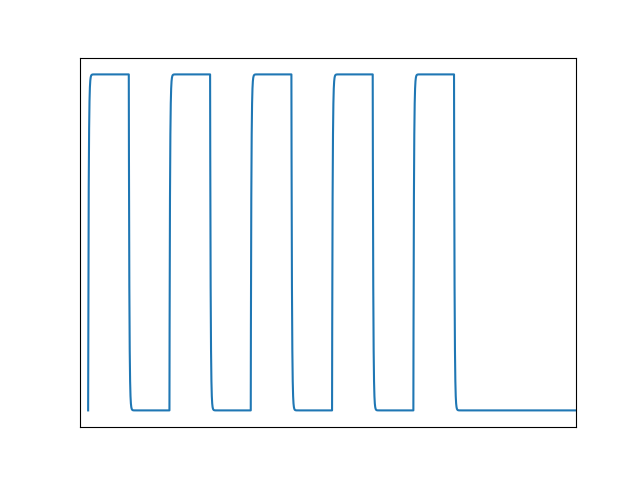
\includegraphics[ width=0.5\textwidth]{./figs/greater_burst_sim.png}}
    \caption{$T = 0.5 s\gg RC$}
\end{figure*}

\begin{comment}
Continous $\hspace{\fill}$ Burst \brak{\text{5 cycles}} $\hspace{\fill}$ Simulation $\hspace{0.5in}$
\begin{figure*}[!htb]
    {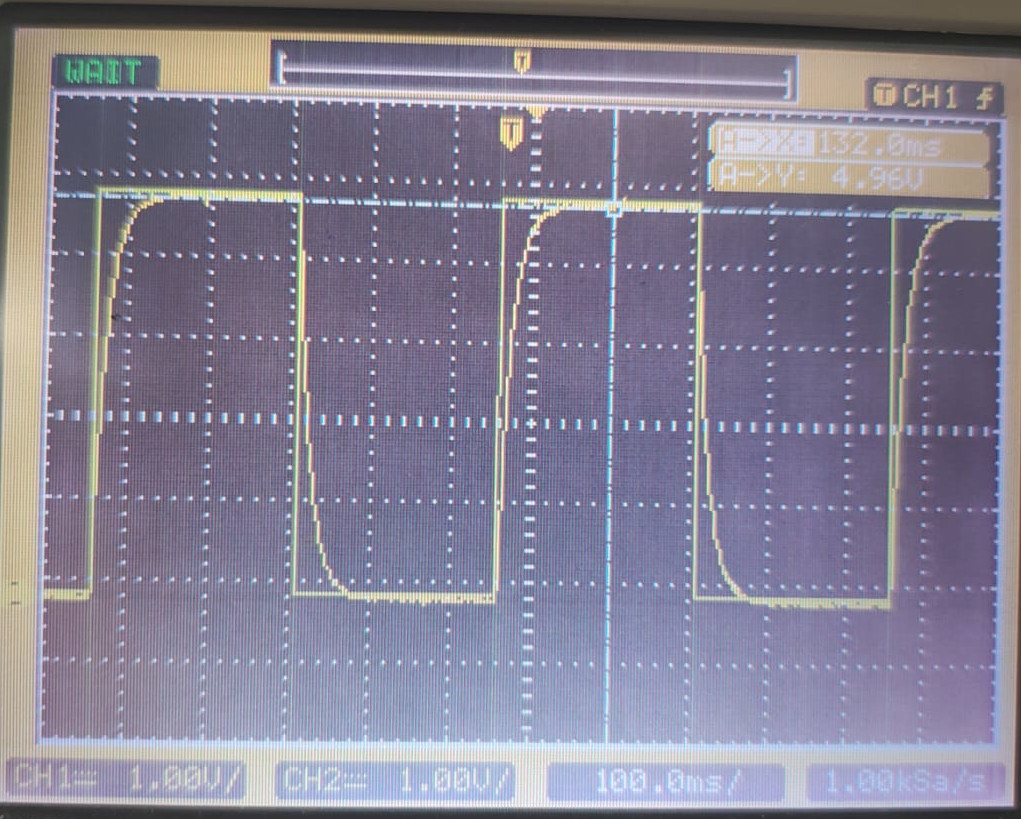
\includegraphics[ width=0.31\textwidth]{./figs/greater_cont_crop.jpeg}}
    \hspace{\fill}
    {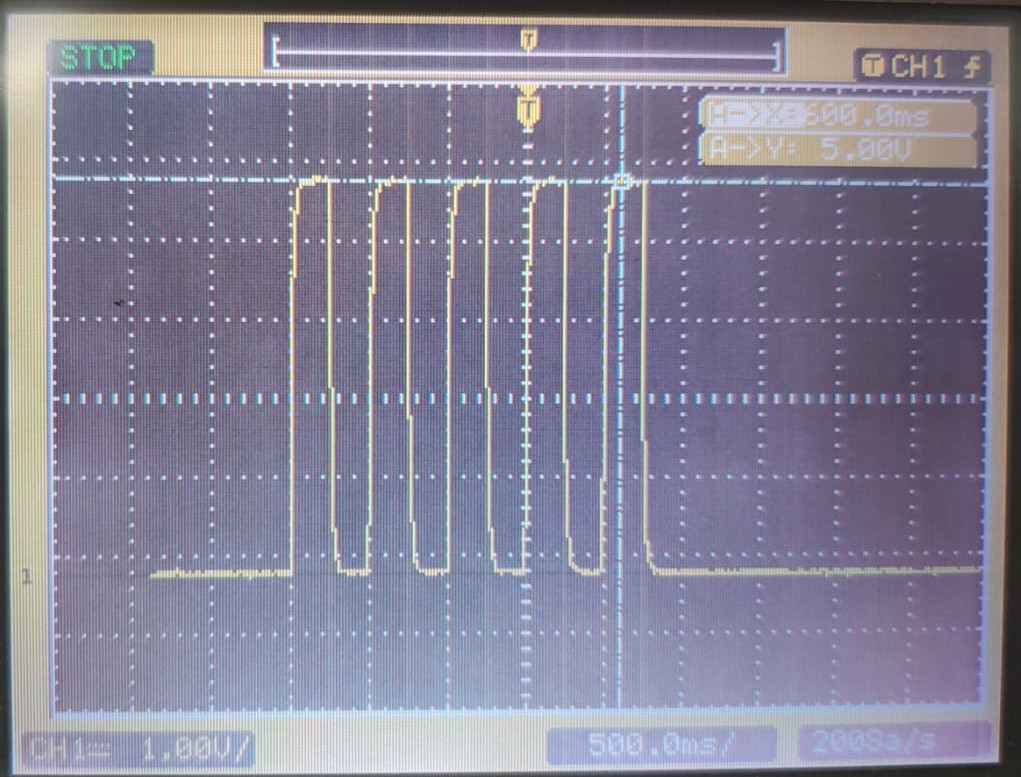
\includegraphics[ width=0.31\textwidth]{./figs/greater_burst_crop.jpeg}}
    \hspace{\fill}
    {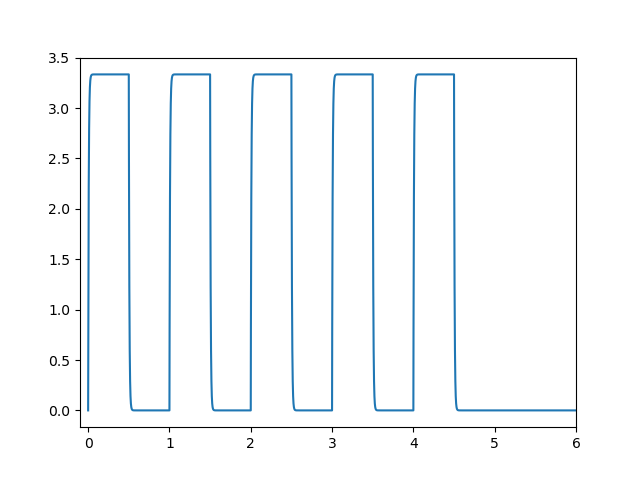
\includegraphics[ width=0.31\textwidth]{./figs/fig2.png}}
    \caption{$T = 0.5 s\gg RC$}
\end{figure*}
\end{comment}

\subsection{Case 2: $T = RC$}
When the period of the square wave is comparable to the time constant ($T \approx RC$), the capacitor does not fully charge or discharge during each half-cycle. The output voltage exhibits noticeable attenuation and rounded transitions, reflecting an intermediate behavior. Inititally we will have the transient response but it will become 0 eventually.
\newpage
Continous $\hspace{\fill}$ Simulation $\hspace{1in}$
\FloatBarrier
\begin{figure*}[!htb]
    {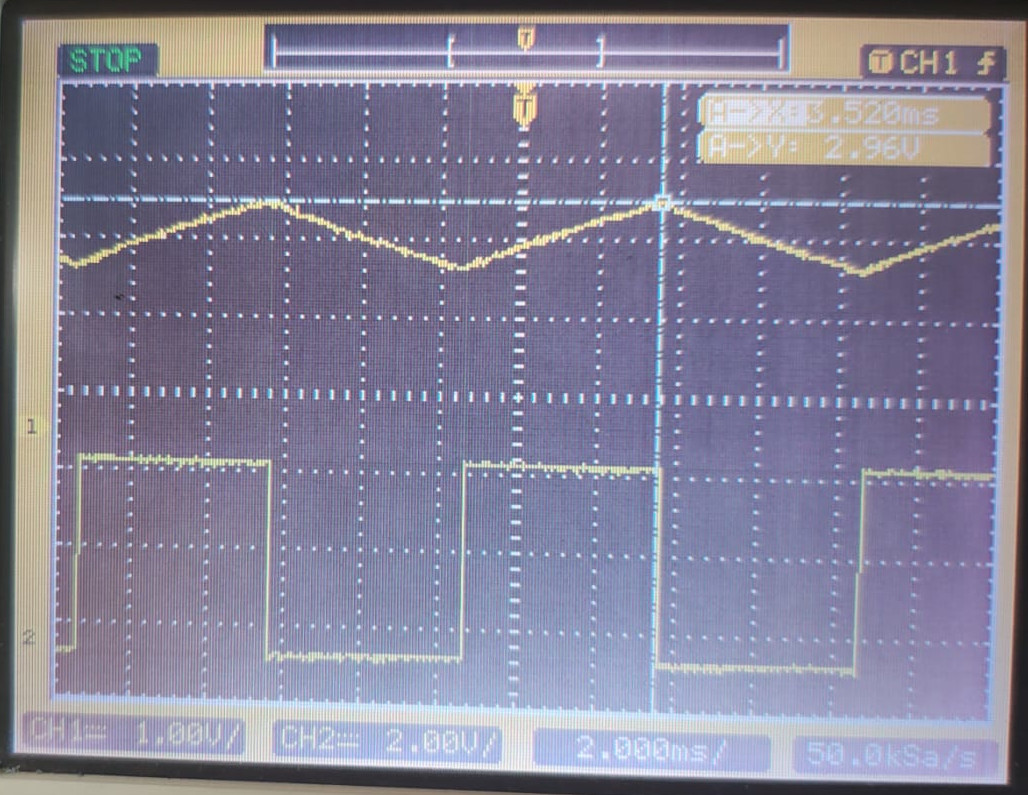
\includegraphics[ width=0.5\textwidth]{./figs/equals_cont_crop.jpeg}}
    \hspace{\fill}
    {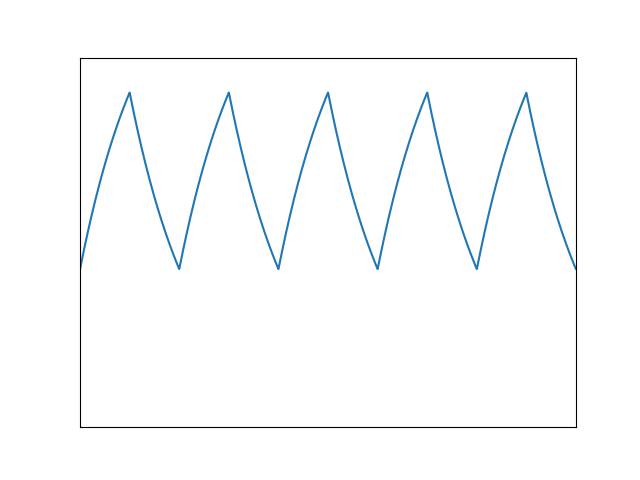
\includegraphics[ width=0.5\textwidth]{./figs/equals_cont_sim.png}}
    \caption{$T = RC = 10^{-2} s$}
\end{figure*}

Burst \brak{\text{5 cycles}} $\hspace{\fill}$ Simulation $\hspace{1in}$
\FloatBarrier
\begin{figure*}[!htb]
    {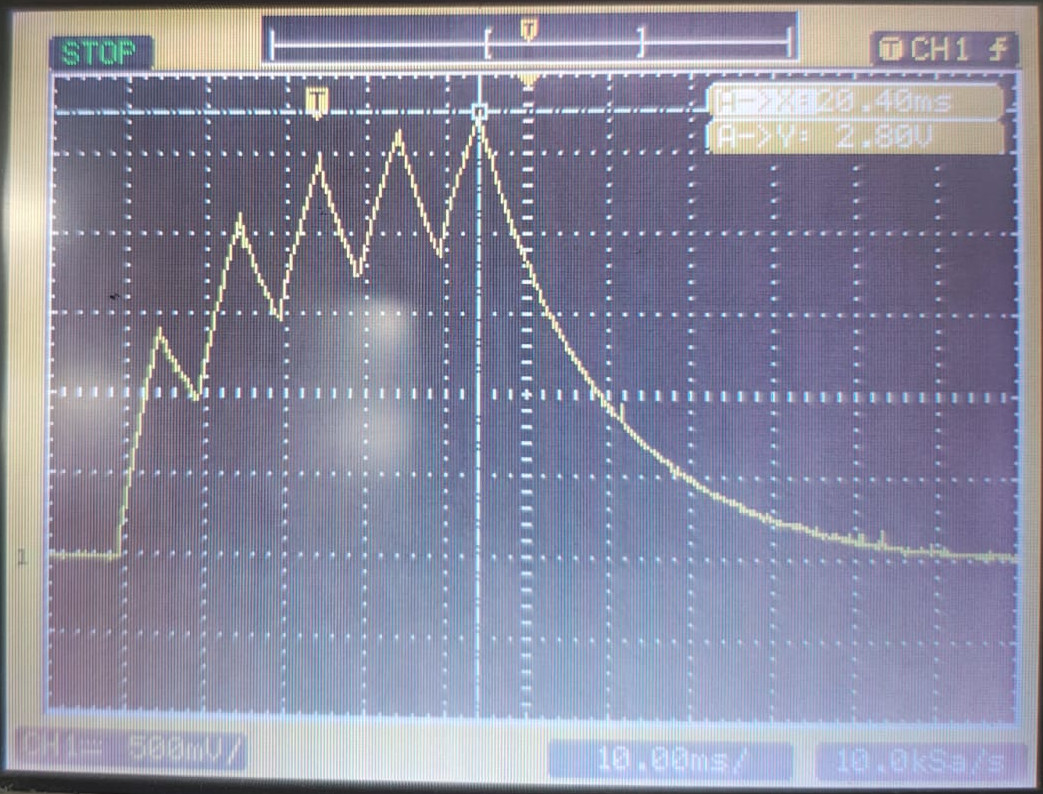
\includegraphics[ width=0.5\textwidth]{./figs/equal_burst_crop.jpeg}}
    \hspace{\fill}
    {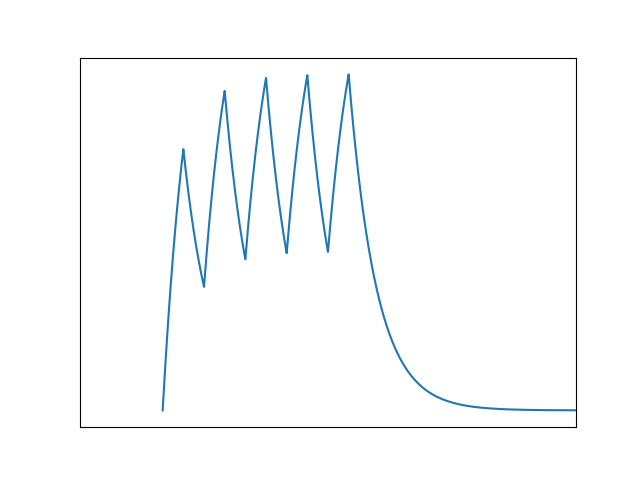
\includegraphics[ width=0.5\textwidth]{./figs/equals_burst_sim.png}}
    \caption{$T = RC = 10^{-2} s$}
\end{figure*}

\subsection{Case 3: $T \ll RC$}
For a square wave with a period much smaller than the time constant ($T \ll RC$), the capacitor cannot respond significantly within a single cycle. The output voltage $V_C(t)$ remains nearly constant, approximating the average value of the input signal. This behavior effectively acts as a low-pass filter, smoothing the square wave into a nearly constant DC level as time progress. Initially, it will grow to a certain value and then oscillates near that level.
\newpage
Continous $\hspace{\fill}$ Simulation $\hspace{1in}$
\FloatBarrier
\begin{figure*}[!htb]
    {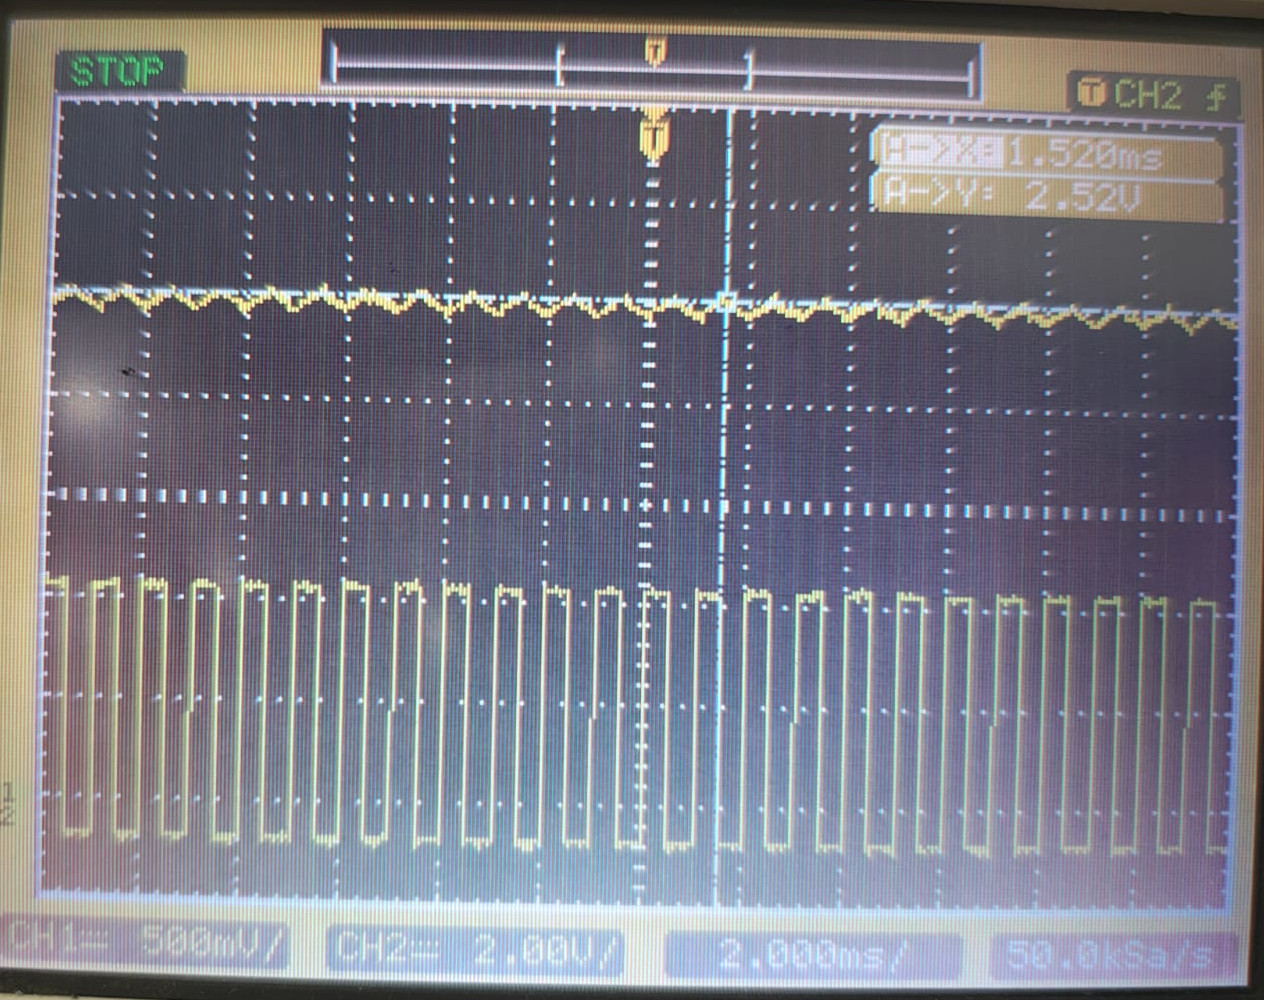
\includegraphics[ width=0.5\textwidth]{./figs/lesser_cont_crop.jpeg}}
    \hspace{\fill}
    {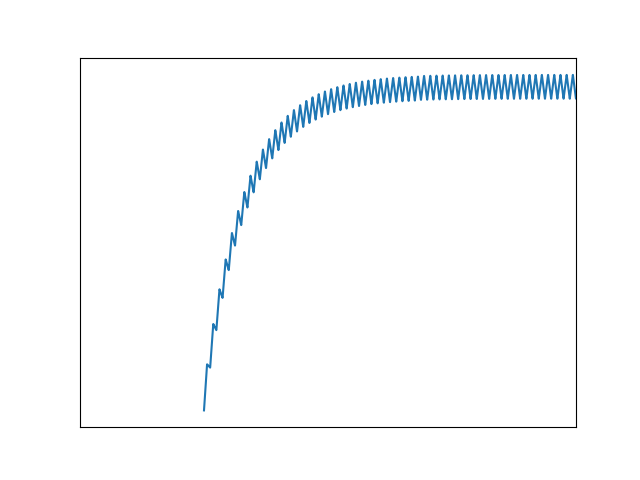
\includegraphics[ width=0.5\textwidth]{./figs/lesser_cont_sim.png}}
    \caption{$T = 10^{-3} s\ll RC$}
\end{figure*}

Burst \brak{\text{5 cycles}} $\hspace{\fill}$ Simulation $\hspace{1in}$
\FloatBarrier
\begin{figure*}[!htb]
    {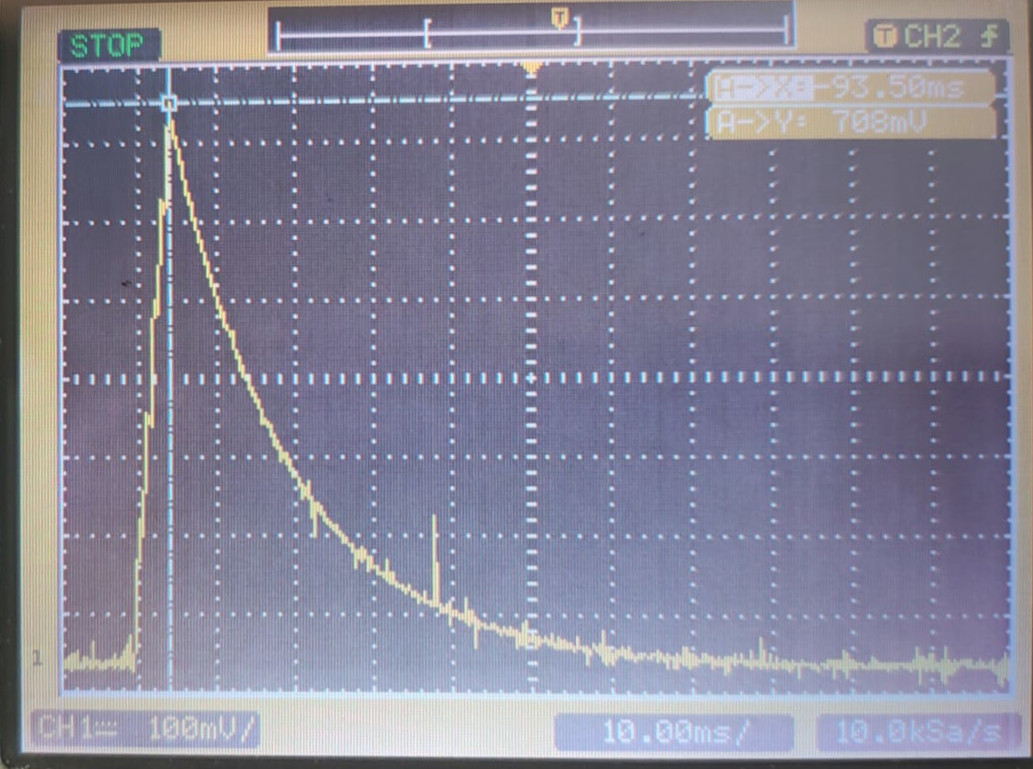
\includegraphics[ width=0.5\textwidth]{./figs/lesser_burst_crop.jpeg}}
    \hspace{\fill}
    {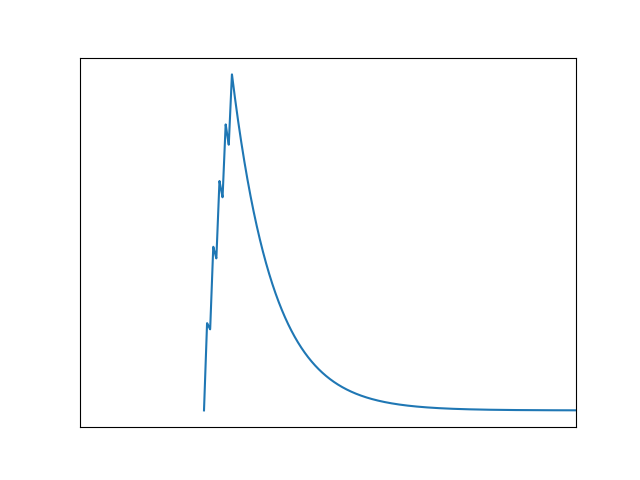
\includegraphics[ width=0.5\textwidth]{./figs/lesser_burst_sim.png}}
    \caption{$T = 10^{-3} s\ll RC$}
\end{figure*}

\section{Verification Codes}
Python verification codes are provided below,
\newline
\url{https://github.com/AbhimanyuKoushik/Lab_reports/blob/main/Lab2/codes/response.py}

\section{Conclusion}
The analysis and numerical simulation confirm that the RC circuit behaves as a filter when subjected to a square wave input. Depending on the relationship between $T$ and $RC$, the circuit either follows the input closely, exhibits attenuation, or behaves as a low-pass filter. The numerical solution using the trapezoidal method effectively captures these behaviors and provides insights into the circuit's transient response.

\end{document}

